% =====================================================================
% THIS FILE IS THE SOURCE. Edit it, then rebuild the PDF with:
%     bash tools/compile.sh Unit_09_Normal_and_the_CLT
% (run from the Course_Rewrite folder; it compiles twice and reports
%  page count, overfull boxes, and em dashes)
%
% Do not edit the PDF directly. Figures are the fig_*.pdf files in this
% folder, regenerated by tools/make_module*_slide_figs.py.
%
% Originally converted from the 15-module draft by a one-shot script now
% parked in tools/one_shot_generators/. Re-running those would discard
% anything you change here, so they are kept out of tools/ on purpose.
% =====================================================================
\documentclass[aspectratio=169]{beamer}
\usetheme{default}
\usefonttheme{professionalfonts}
\usepackage{amsmath, amssymb, amsfonts}
\usepackage{graphicx}
\usepackage{booktabs}
\usepackage{bm}
\usepackage{hyperref}

\mode<presentation> {
    \usetheme{Frankfurt}
    \usecolortheme{default}
}

\newcommand{\xbar}{\bar{x}}
\newcommand{\yhat}{\hat{y}}
\newcommand{\E}[1]{E[#1]}
\newcommand{\SD}[1]{\mathrm{SD}(#1)}

\newenvironment{principle}[1]{\begin{block}{\textbf{Principle:} #1}}{\end{block}}
\newenvironment{trap}[1]{\begin{alertblock}{\textbf{Trap:} #1}}{\end{alertblock}}
\newenvironment{practice}[1]{\begin{exampleblock}{\textbf{In practice:} #1}}{\end{exampleblock}}
\newenvironment{interview}[1]{\begin{exampleblock}{\textbf{You may be asked:} #1}}{\end{exampleblock}}
\newenvironment{yourturn}[1]{%
  \setbeamercolor{block title}{fg=white,bg=orange!80!black}%
  \setbeamercolor{block body}{bg=orange!12}%
  \begin{block}{\textbf{Your turn:} #1}}{\end{block}}
\newenvironment{livedemo}[1]{%
  \setbeamercolor{block title}{fg=white,bg=teal!80!black}%
  \setbeamercolor{block body}{bg=teal!12}%
  \begin{block}{\textbf{Live demo:} #1}}{\end{block}}
\newenvironment{llmcheck}[1]{%
  \setbeamercolor{block title}{fg=white,bg=violet!75!black}%
  \setbeamercolor{block body}{bg=violet!10}%
  \begin{block}{\textbf{LLM check:} #1}}{\end{block}}

\title{The Normal Distribution and the Central Limit Theorem}
\subtitle{Unit 9: Why Averages Are Tame Even When the World Is Not}
\author{Stat 220 \textbar{} Statistics for Data Science}
\date{}

\begin{document}

\begin{frame}
  \titlepage
\end{frame}

% ======================================================================
\section{Why}
% ======================================================================
\begin{frame}{Where this fits}
\begin{itemize}
  \item Since Unit 1 we have written $\text{estimate} \pm 2 \times \text{SE}$ and moved on. This
        unit is where that gets earned.
  \item The claim we have been leaning on is that an \emph{estimate}, a mean or a difference or a
        slope, has a distribution that is close to normal, almost regardless of what the data
        looks like.
  \item That claim is the central limit theorem, and it is the reason a single formula covered
        every test and interval in Part I.
\end{itemize}
\begin{principle}{the debt comes due}
The bell curve is not common because nature loves it. It is common because \emph{adding things up}
produces it, and an average is a sum.
\end{principle}
\end{frame}

\begin{frame}{Live experiment: build a sampling distribution with your hands}
\begin{livedemo}{the class becomes the simulation}
Everyone gets the same printed list of 200 house prices. It is badly right-skewed: mostly
modest homes, a few mansions.
\begin{enumerate}
  \item \textbf{Round 1:} close your eyes, point at \textbf{one} price. Write it down.
  \item \textbf{Round 2:} pick \textbf{ten} prices at random and write down their \emph{average}.
\end{enumerate}
Come to the board and put a sticky note in the right bin: Round 1 values on the top axis, Round 2
averages on the bottom.
\end{livedemo}
\vspace{0.2em}
{\tiny\textit{Materials: the printed price handout (\texttt{Unit\_03\_Price\_Handout.pdf}), sticky notes, a board with two labeled axes. Time: 15 minutes.}}
\centering\small Before we look: predict which histogram will be more symmetric, and which will be
wider.
\end{frame}

\begin{frame}{Stay here while they stick: what will happen}
\begin{itemize}
  \item The \textbf{top} histogram will look like the population: skewed, with a long right tail
        of mansions.
  \item The \textbf{bottom} histogram will be roughly symmetric, bell-shaped, and about
        $\sqrt{10} \approx 3.2$ times narrower.
  \item Nobody coordinated this. Averaging did it.
\end{itemize}
\begin{practice}{what the demo is really about}
``Does my data have to be normally distributed to run a $t$-test?'' The answer lives in the
difference between those two histograms.
\end{practice}
\end{frame}

\begin{frame}{The reveal: the same thing, simulated 20,000 times}
\begin{center}
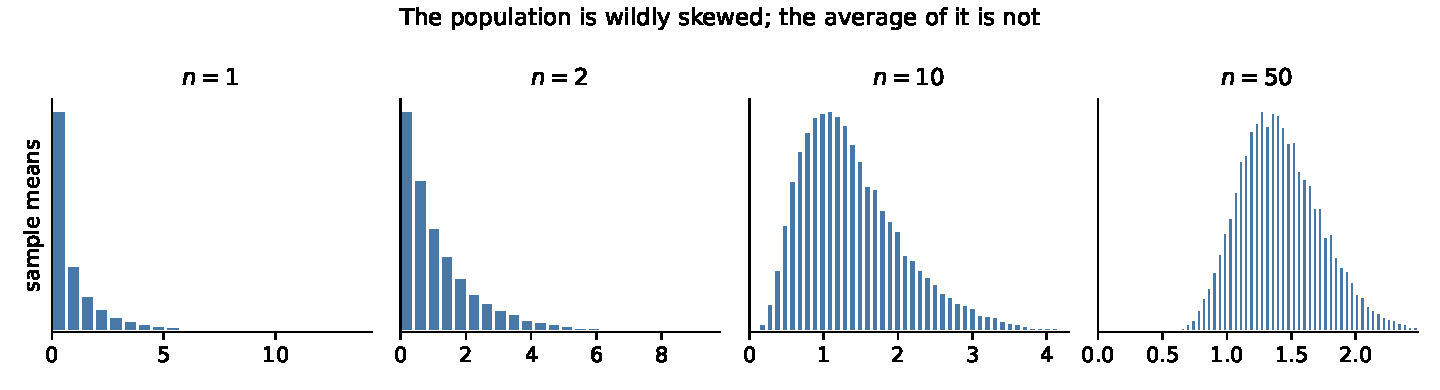
\includegraphics[width=0.95\textwidth]{fig_m07_clt.pdf}
\end{center}
\vspace{-0.3em}
\small The population on the left is severely skewed. By $n = 10$ the average is already nearly
symmetric, and by $n = 50$ it is a textbook bell. Notice also how the width collapses.
\end{frame}

\begin{frame}{What this unit gives you}
\begin{columns}[T]
\begin{column}{0.5\textwidth}
\textbf{Things to know}
\begin{itemize}\small
  \item densities, and why $P(X = x) = 0$ for a continuous variable
  \item the normal distribution, $z$-scores, and 68--95--99.7
  \item the central limit theorem: what it promises and what it does not
  \item the standard error $\sigma/\sqrt{n}$, and why it drives every interval
  \item when the CLT is slow or useless: heavy tails, rare events, dependence
\end{itemize}
\end{column}
\begin{column}{0.5\textwidth}
\textbf{Mistakes to stop making}
\begin{itemize}\small
  \item testing the raw data for normality when the assumption is about the \emph{estimate}
  \item quoting ``$n > 30$'' as if it were a law
  \item using 68--95--99.7 on skewed or heavy-tailed data
  \item confusing the SD of the data with the SE of an estimate
  \item counting rows when the observations are clustered
\end{itemize}
\end{column}
\end{columns}
\end{frame}

% ======================================================================
\section{Continuous variables}
% ======================================================================
\begin{frame}{From bars to curves}
\begin{itemize}
  \item For a continuous quantity (time, price, temperature) there are infinitely many possible
        values, so any exact value has probability zero.
  \item Instead we use a \textbf{density}: probability is the \emph{area} under the curve between
        two points.
  \item ``The chance a call lasts exactly 4.00000 minutes'' is zero. ``Between 3 and 5 minutes''
        is a real number, and it is an area.
\end{itemize}
\begin{principle}{ask for intervals, not points}
Every meaningful question about a continuous variable is a question about a range. This is also
why we report intervals rather than points when we estimate.
\end{principle}
\end{frame}

\begin{frame}{The normal distribution}
Two parameters do all the work: the mean $\mu$ (where it sits) and the SD $\sigma$ (how wide).
\begin{columns}[c]
\begin{column}{0.6\textwidth}
\centering
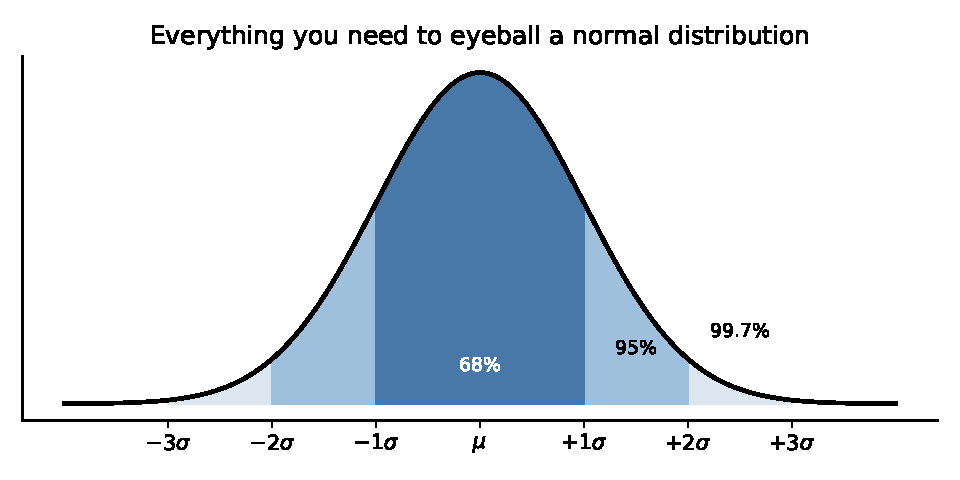
\includegraphics[width=\textwidth]{fig_m07_zrule.pdf}
\end{column}
\begin{column}{0.4\textwidth}
\small
\begin{itemize}
  \item About \textbf{68\%} within $1\sigma$.
  \item About \textbf{95\%} within $2\sigma$.
  \item About \textbf{99.7\%} within $3\sigma$.
\end{itemize}
Memorize these three numbers. They let you sanity-check any claim in your head.
\end{column}
\end{columns}
\end{frame}

\begin{frame}{How to read a density (it is not a probability)}
\begin{itemize}
  \item The height of the curve is \textbf{not} a probability. It can even exceed 1.
  \item Only \emph{areas} are probabilities. The area under the whole curve is 1, and the area
        between two values is the chance of landing between them.
  \item Think of it as a histogram whose bars have been made infinitely thin: the bar heights stop
        being counts, but the area of a region still tells you what fraction lives there.
\end{itemize}
\begin{principle}{the practical consequence}
Never ask ``what is the probability that a call lasts exactly 4 minutes?'' (it is zero). Ask for a
range, or for a percentile. Every real question about a continuous quantity is one of those two.
\end{principle}
\end{frame}

\begin{frame}{The $z$-score: a universal ruler}
\[
z = \frac{x - \mu}{\sigma} \quad\text{``how many standard deviations from the middle?''}
\]
\begin{itemize}
  \item $z$ has no units, so it compares things measured on different scales: a test score, a
        response time, a revenue figure.
  \item $|z| > 2$ is noteworthy, and $|z| > 3$ is rare, \emph{if} the distribution really is normal.
  \item You have already met this: every $t$-statistic in this course is a $z$-score in disguise,
        ``estimate minus null, divided by its standard error.''
\end{itemize}
\begin{principle}{the signal-to-noise template returns}
$\dfrac{\text{how big is the effect}}{\text{how much does it wobble}}$. That ratio is the whole
of inference, and $z$ is its simplest form.
\end{principle}
\end{frame}

\begin{frame}{Your turn \#1}
\begin{yourturn}{read a $z$-score out loud}
A logistics team says delivery times average 40 minutes with a standard deviation of 8 minutes.
A customer's package took 70 minutes.
\vspace{0.3em}

With a neighbor: compute the $z$-score, say how unusual it is if times were normal, and then give
one reason the ``if normal'' clause might be doing a lot of work here.
\end{yourturn}
\end{frame}

\begin{frame}{Your turn \#1: answer}
\begin{itemize}
  \item $z = (70 - 40)/8 = 3.75$. Under a normal model that is about a 1-in-10{,}000 delivery.
  \item But delivery times are \textbf{right-skewed}: traffic, weather, and failed handoffs create
        a long tail that a normal model does not have.
  \item So the honest reading is: unusual, but nowhere near one in ten thousand. The normal model
        is understating the tail.
\end{itemize}
\begin{trap}{sigma-counting on the wrong distribution}
The 68--95--99.7 rule is a property of the normal curve, not of data in general. On skewed data it
will call ordinary events miracles.
\end{trap}
\end{frame}

\begin{frame}{Three quick $z$-scores}
\small
\begin{center}
\begin{tabular}{p{0.36\textwidth} c c p{0.30\textwidth}}
\toprule
\textbf{Situation} & \textbf{value} & $z$ & \textbf{read it as} \\
\midrule
Server response time, mean 220ms, SD 40ms & 300ms & $+2.0$ & slow, but a few percent of
requests will be \\
Exam score, mean 74, SD 9 & 92 & $+2.0$ & same $z$, unrelated units \\
Daily revenue, mean \$40k, SD \$6k & \$22k & $-3.0$ & a genuinely bad day, \emph{if} revenue is
symmetric \\
\bottomrule
\end{tabular}
\end{center}
\vspace{0.4em}
\begin{principle}{why standardizing is worth the trouble}
$z$ strips the units off, so a response time and an exam score become comparable. Every test
statistic in this course is a $z$-score with a different denominator.
\end{principle}
\end{frame}

% ======================================================================
\section{The CLT}
% ======================================================================
\begin{frame}{The central limit theorem}
If $X_1, \ldots, X_n$ are independent draws from \emph{any} distribution with a finite mean $\mu$
and SD $\sigma$, then for large enough $n$:
\[
\xbar \;\approx\; \text{Normal}\!\left(\mu, \; \frac{\sigma}{\sqrt{n}}\right).
\]
\begin{itemize}
  \item The shape of the original distribution does not appear anywhere in that statement.
  \item $\sigma/\sqrt{n}$ is the \textbf{standard error}: the typical distance between your sample
        mean and the truth.
\end{itemize}
\begin{principle}{this is why statistics works at all}
We rarely know the distribution of what we measure. We do not need to. We only need the
distribution of our \emph{estimate}, and that one is predictable.
\end{principle}
\end{frame}

\begin{frame}{The distinction that everything hinges on}
\begin{itemize}
  \item \textbf{Not required:} that your data is normally distributed. Income, charges, and
        durations never are.
  \item \textbf{Required:} that your \emph{estimate} (a mean, a difference, a coefficient) has an
        approximately normal sampling distribution.
  \item The CLT converts the second requirement into a condition about sample size and skew, not
        about the data's shape.
\end{itemize}
\begin{practice}{the sentence worth being able to say}
``The $t$-test does not assume the data is normal. It assumes the sampling distribution of the
mean is roughly normal, which the CLT delivers unless $n$ is small or the data is extremely
skewed.''
\end{practice}
\end{frame}

\begin{frame}{The standard error, and the $\sqrt{n}$ tax}
\[
\SD{\xbar} = \frac{\sigma}{\sqrt{n}}
\]
\begin{itemize}
  \item To halve your uncertainty you need \textbf{four times} the data. To cut it by ten, a
        hundred times.
  \item That is the arithmetic behind every ``can we just collect more data?'' conversation.
  \item It also explains why small samples produce such wild extremes, which is exactly the law of
        small numbers from the probability module.
\end{itemize}
\begin{principle}{precision is expensive and predictable}
Before running a study, use $\sigma/\sqrt{n}$ to work out what precision your budget buys. That is
the entire content of a power calculation.
\end{principle}
\end{frame}

\begin{frame}{Standard deviation versus standard error}
\begin{columns}[T]
\begin{column}{0.48\textwidth}
\textbf{Standard deviation} ($\sigma$ or $s$)
\begin{itemize}\small
  \item spread of the \textbf{individual values}
  \item ``how different are two random customers?''
  \item does \emph{not} shrink with more data: a bigger sample estimates it better but does not
        make it smaller
\end{itemize}
\end{column}
\begin{column}{0.48\textwidth}
\textbf{Standard error} ($\sigma/\sqrt{n}$)
\begin{itemize}\small
  \item spread of your \textbf{estimate}
  \item ``how far is my sample mean from the truth?''
  \item shrinks like $1/\sqrt{n}$
\end{itemize}
\end{column}
\end{columns}
\vspace{0.4em}
\begin{trap}{the error that produces absurd intervals}
Using $s$ where you needed $s/\sqrt{n}$ (or the reverse) is the single most common technical
mistake students make all semester. Ask yourself out loud: \emph{am I describing people, or
describing my estimate?}
\end{trap}
\end{frame}

\begin{frame}{Four things the CLT does not say}
\begin{itemize}
  \item It does \textbf{not} say your data becomes normal. A bigger sample of incomes is still
        a pile of skewed incomes.
  \item It does \textbf{not} help with a \emph{single} observation. Predicting one customer is
        governed by $\sigma$, not by $\sigma/\sqrt{n}$.
  \item It does \textbf{not} fix bias. If your sample is drawn from the wrong population, the
        average of it converges beautifully to the wrong number.
  \item It does \textbf{not} apply to every statistic. The sample maximum, for instance, never
        becomes normal no matter how much data you collect.
\end{itemize}
\begin{principle}{what it does say}
Sums and averages of many independent, not-too-extreme pieces are approximately normal. That is
narrow, and it is enough to build the whole course on.
\end{principle}
\end{frame}

\begin{frame}{How large is ``large enough''? It depends on the skew}
\begin{center}
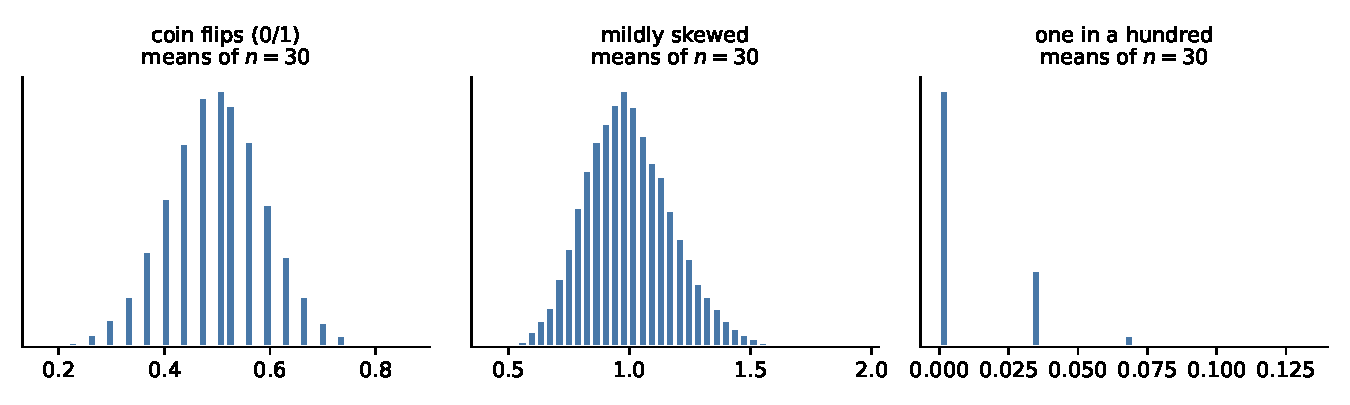
\includegraphics[width=0.95\textwidth]{fig_m07_howbig.pdf}
\end{center}
\vspace{-0.4em}
\small
All three show means of $n = 30$. Coin flips are already perfect. Mild skew is fine. But a
1-in-100 rare event at $n = 30$ is still hopeless: most samples contain zero events, and the
average is lumpy, not bell-shaped.
\end{frame}

\begin{frame}{Retire the ``$n > 30$'' rule}
\begin{itemize}
  \item $n = 30$ is plenty for symmetric data, marginal for moderately skewed data, and useless
        for rare events or heavy tails.
  \item A workable rule for proportions: you want at least about 10 successes \emph{and} 10
        failures, not just 30 rows.
  \item If you are unsure, do not argue about rules: \textbf{bootstrap} the estimate and look at
        the shape of its distribution directly.
\end{itemize}
\begin{trap}{a rule of thumb quoted as a law}
``$n > 30$ so the CLT applies'' is the most confidently repeated wrong sentence in applied
statistics. The right question is always: how skewed, and how rare?
\end{trap}
\end{frame}

\begin{frame}{Your turn \#2}
\begin{yourturn}{is the CLT going to save you?}
Three analyses, each with $n = 40$:
\begin{enumerate}
  \item average height of 40 students
  \item average purchase amount of 40 customers, where one bought a \$45{,}000 tractor
  \item fraction of 40 users who clicked, when the click rate is about 0.5\%.
\end{enumerate}
With a neighbor: for each, will the sample mean be roughly normal? Rank them from safest to
most dangerous.
\end{yourturn}
\end{frame}

\begin{frame}{Your turn \#2: answer}
\begin{itemize}
  \item \textbf{Heights} (safest): nearly symmetric already, so $n = 40$ is more than enough.
  \item \textbf{Purchases}: one enormous value dominates the mean. The sampling distribution is
        skewed and the SE is unstable. Report a median, or bootstrap, or model the tail.
  \item \textbf{Clicks} (most dangerous): with 0.5\% and $n = 40$ you expect \emph{0.2} clicks.
        There is no meaningful normal approximation. You need thousands of users, or an exact
        binomial method.
\end{itemize}
\begin{principle}{the CLT is about the effective number of informative observations}
Forty rows containing one event is not a sample of forty.
\end{principle}
\end{frame}

% ======================================================================
\section{When normal fails}
% ======================================================================
\begin{frame}{Real data is not normal, and that is fine}
\begin{center}
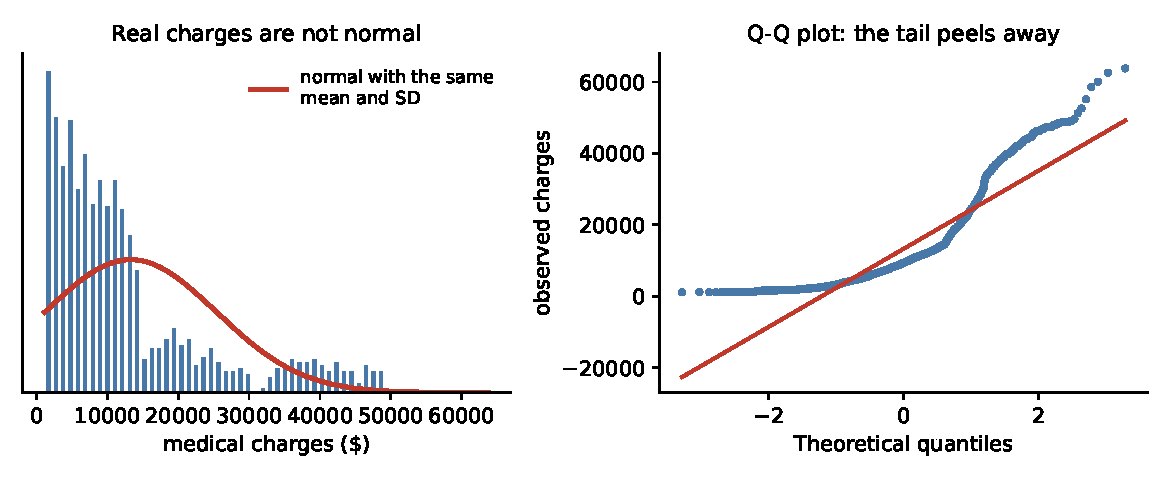
\includegraphics[width=0.92\textwidth]{fig_m07_realdata.pdf}
\end{center}
\vspace{-0.4em}
\small
Medical charges for 1{,}338 people. The normal curve with the same mean and SD predicts negative
charges and misses the entire right tail. The Q-Q plot shows the tail peeling away from the line.
None of this stops us from estimating the \emph{mean} charge with a normal-based interval.
\end{frame}

\begin{frame}{Reading a Q-Q plot in five seconds}
\begin{itemize}
  \item Points on the line: consistent with normal.
  \item Both ends curving \textbf{up} above the line on the right: a long right tail (money,
        durations, city sizes).
  \item An S-shape: heavy tails on both sides, so extremes are more common than normal predicts.
  \item Steps or gaps: the variable is discrete or has been rounded or censored.
\end{itemize}
\begin{principle}{diagnose, do not just test}
A normality \emph{test} gives you a $p$-value that is useless at both extremes: it rejects
harmless deviations in huge samples and misses real ones in small samples. Look at the picture
instead.
\end{principle}
\end{frame}

\begin{frame}{The log-normal: when things multiply}
\begin{itemize}
  \item The CLT says sums of many small effects become normal. If effects \emph{multiply} instead
        of adding, the logarithm becomes normal and the variable is \textbf{log-normal}.
  \item Income, revenue per customer, insurance claims, city sizes, and stock prices are all
        roughly log-normal, because growth compounds.
  \item That is why taking logs so often fixes a skewed regression: it converts a multiplicative
        world into an additive one.
\end{itemize}
\begin{practice}{a useful way to say it}
``Money is usually log-normal, not normal, because it grows by percentages rather than by
increments.''
\end{practice}
\end{frame}

\begin{frame}{Heavy tails: where the argument breaks entirely}
\begin{columns}[c]
\begin{column}{0.58\textwidth}
\centering
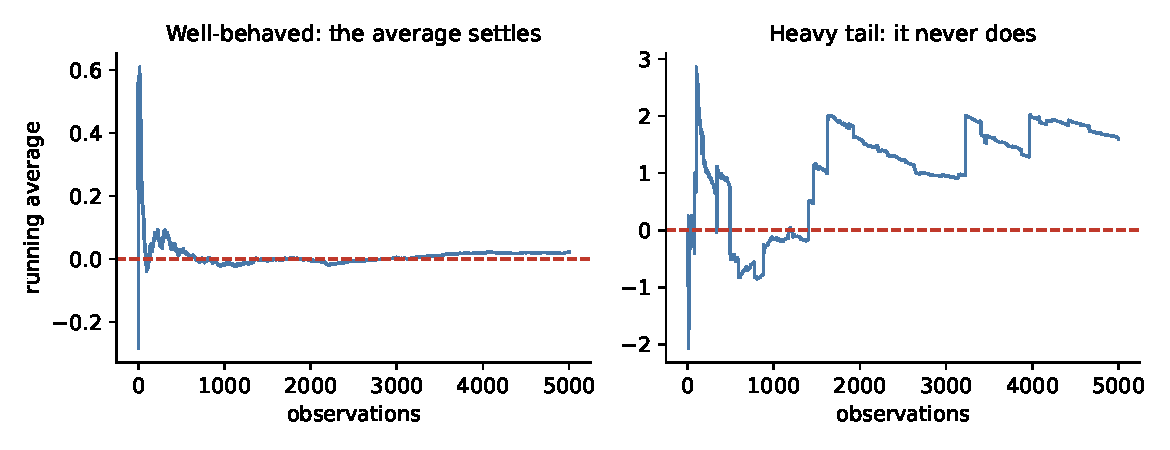
\includegraphics[width=\textwidth]{fig_m07_heavytail.pdf}
\end{column}
\begin{column}{0.42\textwidth}
\small
On the left, a well-behaved variable: the running average locks onto the truth.
\vspace{0.4em}

On the right, a heavy-tailed one: every so often a single enormous draw resets the average. It
never converges, because the theoretical mean does not exist.
\end{column}
\end{columns}
\onslide<2->{\centering\small
Insurance losses, market crashes, and viral traffic live closer to the right panel than anyone
likes.}
\end{frame}

\begin{frame}{Dependence quietly destroys $\sqrt{n}$}
\begin{itemize}
  \item The CLT assumes independent draws. Real data is full of dependence: repeated measurements
        on the same user, days in a row, students in the same class.
  \item With dependence, your \textbf{effective} sample size is far below your row count, so the
        standard error you computed is too small and your interval is too narrow.
  \item Symptom: absurdly tiny $p$-values on data that everyone knows is clustered. You saw this
        in Part 1, with 400{,}000 sessions from two cities.
\end{itemize}
\begin{trap}{counting rows instead of independent units}
Ask ``how many independent things do I really have?'' Often the answer is the number of users, or
stores, or weeks, not the number of rows.
\end{trap}
\end{frame}

\begin{frame}{Your turn \#3}
\begin{yourturn}{which number does the question need?}
Your company's delivery times have mean 42 minutes and SD 15 minutes, measured on 900 deliveries.
For each question, say whether you need the \textbf{SD} or the \textbf{SE}, and compute it:
\begin{enumerate}
  \item ``Roughly what range covers most individual deliveries?''
  \item ``How precisely do we know the average delivery time?''
  \item ``Should we promise every customer delivery within an hour?''
\end{enumerate}
\end{yourturn}
\end{frame}

\begin{frame}{Your turn \#3: answer}
\begin{itemize}
  \item (1) \textbf{SD.} About 95\% of individual deliveries fall within roughly
        $42 \pm 2(15)$, so 12 to 72 minutes. Wide, because people vary.
  \item (2) \textbf{SE.} $15/\sqrt{900} = 0.5$ minutes, so the average is known to about
        $42 \pm 1$ minute. Narrow, because averaging kills noise.
  \item (3) \textbf{SD again}, and it is bad news: an hour is only $z = 1.2$ above the mean, so
        roughly 12\% of deliveries would miss the promise. Knowing the average within a minute
        does not help a single late customer.
\end{itemize}
\begin{principle}{the question to ask yourself}
Am I describing \emph{people}, or describing \emph{my estimate}? Promises to customers need the
SD. Claims about a population average need the SE.
\end{principle}
\end{frame}

% ======================================================================
\section{LLM check}
% ======================================================================
\begin{frame}{LLM check: mistake or not? (1 of 2)}
\begin{llmcheck}{we asked an LLM about an assumption}
\textbf{We told it:} ``Our revenue-per-customer data is very right-skewed. We have 5{,}000
customers. Can we use a $t$-test to compare two groups?''\\[4pt]
\textbf{It answered:} ``No. The $t$-test requires normally distributed data. Since your data is
skewed, you must transform it or use a nonparametric test instead.''
\end{llmcheck}
\vspace{0.2em}
\centering\small Mistake, or no mistake?
\onslide<2->{%
\begin{trap}{verdict: mistake}
The assumption is about the sampling distribution of the \emph{mean}, not the raw data. With
5{,}000 customers per group the CLT handles ordinary skew comfortably. (A transformation might
still be a good idea, but for interpretability or heavy tails, not because the test is invalid.)
\end{trap}}
\end{frame}

\begin{frame}{LLM check: mistake or not? (2 of 2)}
\begin{llmcheck}{same territory, a different answer}
\textbf{We told it:} ``We ran 40 users and 0.5\% typically click. Our A/B test shows a 50\% lift.
Is it significant?''\\[4pt]
\textbf{It answered:} ``With a 0.5\% base rate and 40 users you expect a fraction of one click, so
the normal approximation does not apply and almost no result would be interpretable. I would use
an exact binomial method, and more importantly, I would compute the sample size needed to detect
a 50\% lift, which will be in the tens of thousands.''
\end{llmcheck}
\vspace{0.2em}
\centering\small Mistake, or no mistake?
\onslide<2->{%
\begin{principle}{verdict: no mistake}
It recognized that $n = 40$ is not $n = 40$ when the event is rare, refused the approximation, and
redirected to the real question: how much data would this take?
\end{principle}}
\end{frame}

% ======================================================================
\section{Workflow}
% ======================================================================
\begin{frame}{Deciding whether your normal-based answer is safe}
\begin{enumerate}
  \item \textbf{Name the estimate}, not the data: is it a mean, a difference, a proportion, a
        coefficient?
  \item \textbf{Plot the raw data} once, to see skew, gaps, and outliers. Do not test it.
  \item \textbf{Count the informative observations}: successes and failures, not just rows.
  \item \textbf{Ask what is independent}, and reduce $n$ to that.
  \item \textbf{If in doubt, bootstrap} the estimate and look at the shape you actually get.
  \item \textbf{Report the SE and the interval}, and say which assumption is carrying the weight.
\end{enumerate}
\end{frame}

\begin{frame}{Scenario: the outlier that ate the interval}
\textbf{Setup.} An analyst reports average order value of \$310 with a 95\% interval of
\$180 to \$440 from 200 orders. One order was a \$40{,}000 bulk purchase.
\begin{itemize}
  \item That single order dominates both the mean and the SD, so the interval is driven by one
        observation rather than by 200.
  \item Deleting it silently is not an option: bulk orders are real revenue.
  \item Better: report the median alongside the mean, bootstrap the interval, and, if the business
        question is about typical customers, analyze bulk orders as their own segment.
\end{itemize}
\begin{practice}{how to answer this}
``I would ask whether the question is about the total (keep the whale) or the typical customer
(model it separately), and I would use a bootstrap rather than the formula.''
\end{practice}
\end{frame}

% ======================================================================
\section{Consolidate}
% ======================================================================
\begin{frame}{Deciding whether a normal-based answer is safe}
\small
\begin{enumerate}
  \item \textbf{Name the estimate}, not the data: a mean, a difference, a proportion?
  \item \textbf{Plot the raw data once} to see skew, gaps, and outliers. Do not run a normality test.
  \item \textbf{Count the informative observations}, which for a proportion means successes and failures, not rows.
  \item \textbf{Ask what one independent observation is}, and reduce $n$ to that.
  \item \textbf{Convert to a $z$-score} when you need to compare across units: $z=(x-\mu)/\sigma$.
  \item \textbf{If in doubt, simulate.} Resample your own data and look at the shape of the estimate.
  \item \textbf{Report the SE and the interval}, and say which assumption is carrying the weight.
\end{enumerate}
\end{frame}

\begin{frame}{The traps, all in one place}
\begin{trap}{the ones that bite most often}
\begin{itemize}
  \item Requiring the raw data to be normal when the assumption is about the estimate.
  \item Reciting ``$n > 30$'' regardless of skew or rarity.
  \item Applying the 68--95--99.7 rule to skewed or heavy-tailed data.
  \item Treating 3-sigma events as impossible in fat-tailed domains.
  \item Using row counts as $n$ when the observations are clustered or repeated.
  \item Running a normality test and letting its $p$-value make the decision.
\end{itemize}
\end{trap}
\end{frame}

\begin{frame}{Ten questions to be able to answer}
\begin{enumerate}\small
  \item Why is the normal distribution so common?
  \item Does a $t$-test require normally distributed data? Explain carefully.
  \item What is a standard error, and how does it differ from a standard deviation?
  \item How large does $n$ need to be for the CLT to apply?
  \item What does a $z$-score of 3 mean, and when would you not be impressed by one?
  \item Our data is log-normal. What does that suggest about how it was generated?
  \item Why do heavy tails break the usual averaging argument?
  \item We have 100{,}000 rows but only 300 customers. What is our real sample size?
  \item How would you check whether a normal-based interval is trustworthy here?
  \item A colleague deletes outliers until a normality test passes. What do you say?
\end{enumerate}
\end{frame}

\begin{frame}{Mastery checklist}
You have this unit when you can, from memory:
\begin{itemize}
  \item explain density, area as probability, and why point probabilities are zero
  \item compute and interpret a $z$-score, and use 68--95--99.7 to sanity-check claims
  \item state the CLT precisely, including what it assumes
  \item explain why the standard error is $\sigma/\sqrt{n}$ and what that costs you
  \item distinguish normality of the data from normality of the estimate
  \item name three situations where the CLT will not rescue you
\end{itemize}
\end{frame}

\begin{frame}{What you should be able to do with software}
\small
Nobody is asking you to memorize syntax. You are expected to know \emph{which} procedure the
question calls for, what to hand it, and what the output means. With an AI assistant open, you
should be able to produce any of these and defend the result.
\begin{center}\footnotesize
\begin{tabular}{p{0.44\textwidth} p{0.46\textwidth}}
\toprule
\textbf{You should be able to} & \textbf{What you would reach for} \\
\midrule
Normal probabilities and percentiles & \texttt{stats.norm.cdf}, \texttt{stats.norm.ppf} \\
Standardize a value & \texttt{(x - mean) / sd} \\
Check normality by eye & \texttt{stats.probplot}, plus a histogram \\
Build a sampling distribution yourself & \texttt{rng.integers} to resample, then \texttt{.mean(axis=1)} \\
Standard error of a mean & \texttt{s / np.sqrt(n)} \\
Check whether an interval really covers 95\% & simulate many samples and count \\
Measure dependence in a series & \texttt{Series.autocorr(1)} \\
\bottomrule
\end{tabular}
\end{center}
\vspace{0.2em}
\centering\small
If you cannot say what the output means, the fact that you produced it is worth nothing.
\end{frame}

\begin{frame}{Where we go next}
\begin{itemize}
  \item We now know the shape of an estimate's uncertainty. Next: \textbf{estimation itself}, how
        to build a good estimate, judge it, and put an interval around it without leaning on a
        formula.
  \item That module introduces likelihood and the bootstrap, and it is the direct on-ramp to the
        inference material.
\end{itemize}
\begin{principle}{the through-line}
You almost never know the distribution of what you measure. You can almost always know the
distribution of what you estimate. Statistics lives in that gap.
\end{principle}
\end{frame}

\end{document}
